\documentclass[a4paper]{exam}

\usepackage{graphicx}

\usepackage{siunitx}
\DeclareSIUnit{\revolution}{rev}
\DeclareSIUnit{\rpm}{\revolution\per\minute}
\DeclareSIUnit{\lightyear}{ly}

\begin{document}
  \section*{L2 Physics: Problems on waves}
  The speed of sound is \SI{340}{\metre\per\second} in air. See also the final page for useful formulae.
  \subsection*{Sections 1.1-1.2}
  \begin{questions}
    \question A radio station sends out radio waves with frequency \SI{750}{\kilo\hertz}. All radio waves travel with a speed
              of \SI{3.0e8}{\metre\per\second}. How far apart are the crests of the wave sent out by the station?
    \question A television station sends out radio waves with frequency \SI{750}{\mega\hertz}. All radio waves travel with a speed
              of \SI{3.0e8}{\metre\per\second}. How far apart are the crests of the wave sent out by the station?
    \question A wave has wavelength \SI{2}{\centi\metre}; at a given point, 25 wave crests per second are observed. Calculate
              (a) the frequency of the wave; (b) the speed of the wave; (c) the time between observed wave crests.
    \question The wave shown below is travelling to the right with a speed of \SI{2.00}{\metre\per\second}. How long
              after the instant shown will the crest on the left have moved to the position of the crest on the right?

              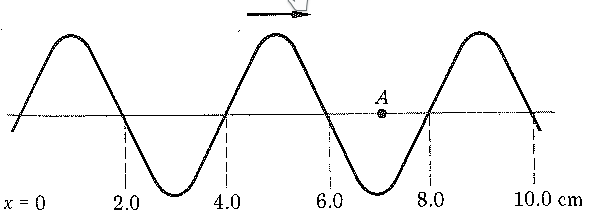
\includegraphics[width=0.4\textwidth]{beuche132}
    \question If the same wave is slowed so that it is moving at a speed of \SI{100}{\centi\metre\per\second}, how many
              crests per second will pass point $ A $?
    \question What frequency must a sound source have if the wavelength of its sound is to be \SI{3.0}{\centi\metre}?
  \end{questions}
  \subsection*{Sections 1.3-1.4}
  \begin{questions}
    \question The two pulses in the igure are moving down the string at \SI{2.0}{\metre\per\second} each. Sketch the position
              of the string (a) after \SI{0.40}{\second}; (b) after \SI{0.20}{\second}.

              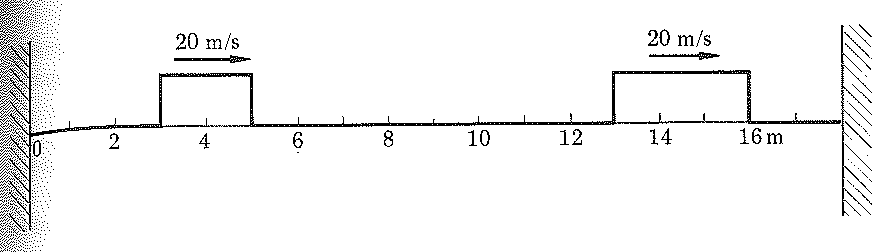
\includegraphics[width=0.4\textwidth]{beuche131}
    \question Two waves moving in opposite directions can interfere with each other in such a way that no net movement is seen;
              this is called an \emph{standing wave}. Give a simple example of an experiment you could set up to show this.
    \question Describe a water-wave experiment which illustrates the phenomenon of diffraction.
    \question Jenna is conducting an experiment; she places a tone generator (a machine that generates a particular frequency
              of wave) on the other side of a narrow slit in a sound-proof barrier. She notices that, if the generator is placed
              around the corner as in the following diagram, the sound of the generator is much louder when it is set to a lower
              frequency. Explain this observation.

              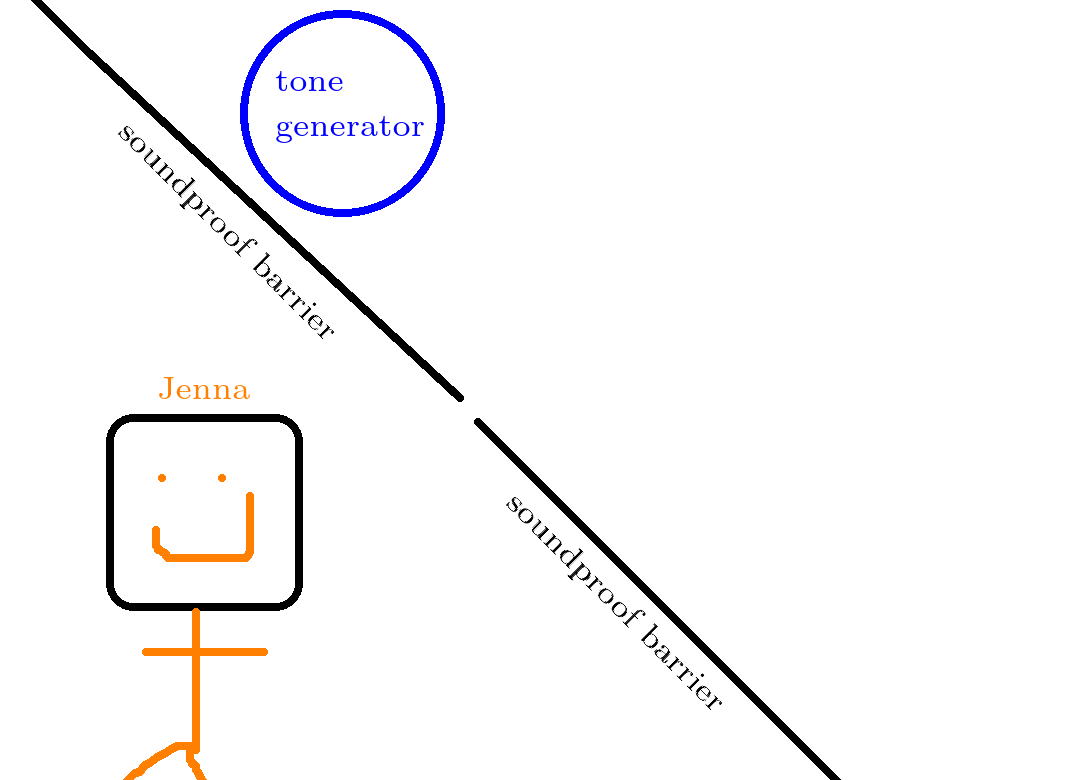
\includegraphics[width=0.4\textwidth]{jenna}
    \question Two identical sound sources are at the coordinate origin and send \SI{70}{\centi\metre} wavelength waves out. One source is
              now moved slowly to the left (to negative $ x$--values). For an observer at point $ x = 20\thinspace\si{\metre} $ on the $ x$--axis,
              what positions of the moving source give rise to (a) the loudest and (b) the quietest observed sound? (Assume the sources
              are in phase.)
    \question Two identical sources with unknown wavelength are on the $ x$--axis some distance apart. One of the sources is moved
              away from the observer (who is also on the $ x$--axis, but some way away).
      \begin{parts}
        \part Draw a diagram and annotate it to explain why the observer hears alternating loud and weak sounds.
        \part If the source moves \SI{30}{\centi\metre} between observed loud sounds, what is the wavelength of the sound?
      \end{parts}
    \question At a given place there are two gaps, labelled $ S_1 $ and $S_2 $, in a line of rocks. A set of waves
              passes through the rocks, creating an interference pattern. The difference between the distance between
              points $ S_1 $ and $ X $, and the distance between $ S_2 $ and $ X $, is \SI{0.40}{\metre}. The wave
              speed is \SI{0.80}{\metre\per\second}, and one reaches the wall each second. Is $ X $ at a node or an antinode?
              Explain your answer.

              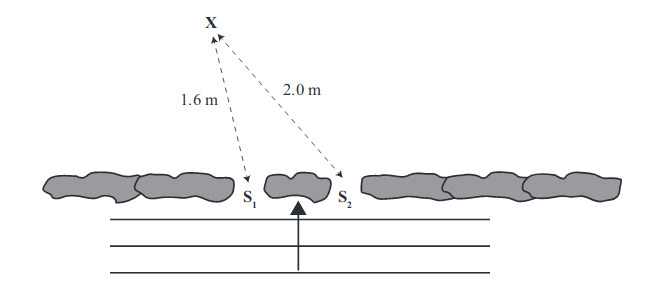
\includegraphics[width=0.4\textwidth]{nzqa20141}
    \question Water waves travel from deep to shallow water. The wave-fronts of the wave hit the boundary between the depths at
              a shallow angle. Draw a diagram showing the relation of the wavefronts leaving the boundary to those reaching it.
              Which phenomenon does your diagram illustrate?

              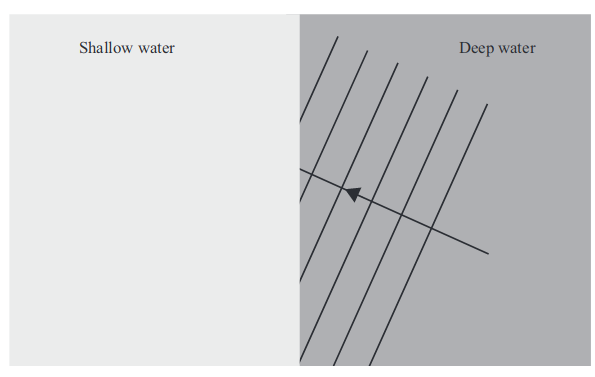
\includegraphics[width=0.4\textwidth]{nzqa20142}
    \question Consider the following systems of waves.

              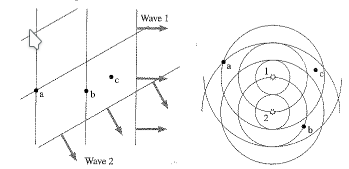
\includegraphics[width=0.4\textwidth]{knight1789}
      \begin{parts}
        \part In the left-hand system, both waves have an amplitude of \SI{2.0}{\milli\metre} and the same wavelength. What
              is the net displacement of the medium at points $ a $, $ b $, and $ c $?
        \part In the right-hand system, both circular waves are in phase. Are $ a $, $ b $, and $ c $ points of maximum constructive
              interference, points of maximum destructive interference, or in between?
      \end{parts}
    \question Noise-cancelling headphones are an application of destructive interference. Each side of the headphones uses a microphone
              to pick up noise, delays it slightly, and then rebroadcasts it to your ear where it can interfere with the incoming sound
              wave of the noise. Suppose you are sitting \SI{1.5}{\metre} from an annoying \SI{120}{\hertz} buzzing sound. What is the
              minimum headphone delay, in milliseconds, that will cancel this noise?
  \end{questions}
  \clearpage
  \section*{Formulae}
  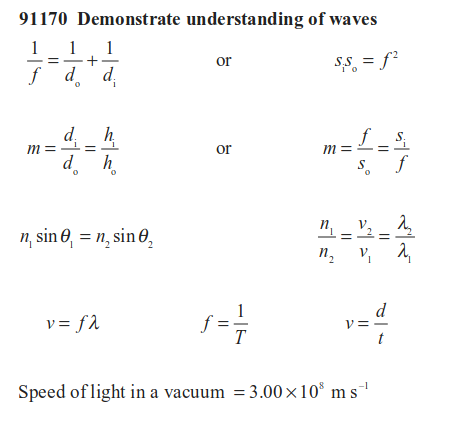
\includegraphics{waves}
\end{document}
